\documentclass[11pt,a4paper,twocolumn]{article}

\usepackage[utf8]{inputenc}
\usepackage[margin=1.8cm]{geometry}
\usepackage{times}
\usepackage{microtype}
\usepackage{amsmath,amssymb}
\usepackage{graphicx}
\usepackage{booktabs}
\usepackage{multirow}
\usepackage{xcolor}
\usepackage{hyperref}
\usepackage{caption}
\usepackage[numbers]{natbib}

\hypersetup{
    colorlinks=true,
    linkcolor=blue!70!black,
    citecolor=blue!70!black,
    urlcolor=blue!70!black
}

\title{\textbf{Whose Words Are Reachable? Human Writing and Frontier LLMs Through the Lens of Smaller Models}}

\author{
  \textbf{Pedro Faustini}$^{1}$ \quad \textbf{WordsGPT Research}$^{2}$ \\
  $^{1}$Macquarie University \quad $^{2}$WordsGPT \\
  \texttt{pedro.faustini@mq.edu.au}
}

\date{}

\begin{document}

\maketitle

\begin{abstract}
When a small open-weight language model reads a text word by word under teacher forcing, how often does the next word fall inside the model's plausible sampling support? We formalize this question with the \textbf{Word Coverage Score (WCS)}, a directional, non-parametric reachability measure that evaluates whether every sub-token of each word in a source text survives a scoring model's candidate-pool filter (such as top-$p$ nucleus truncation over top-$K$ candidates or the model's shipped generation configuration). Evaluating multiple scorers against multiple sources yields an asymmetric \textbf{scorer-by-source reachability matrix}.

We conduct a comprehensive empirical audit across 100 length-controlled prompts spanning two distinct domains---conversational explanations (\textbf{HC3 Reddit ELI5}, 50 prompts) and formal encyclopedic exposition (\textbf{HC3 Wikipedia CS/AI}, 50 prompts)---evaluating \textbf{9 open-weight scorers across 4 model families} (Qwen~3.5, Gemma~4, Llama~3.1/3.2, and Mistral~7B; $1\text{B}$--$27\text{B}$ parameters) against \textbf{18 text sources} organized into human writing and three machine generator tiers: \textbf{Small Open-Weight} ($\le 32\text{B}$), \textbf{Large Open-Weight} ($427\text{B}$--$2.78\text{T}$ total parameters: Qwen3.8-2.4T-A95B, DeepSeek-V4-Pro, DeepSeek-V4.1-Flash, GLM-5.3, Kimi-K3, MiniMax-M3, MiMo-V2.6-Pro), and \textbf{Frontier Proprietary} (GPT-6 Astra, Claude Opus 5.5, Gemini 4 Argon).

Our experiments establish five core findings:
(1) \textbf{A Three-Tier Generator Hierarchy:} Under realistic top-$p=0.99$ scoring on ELI5, small scorers reach small open-weight generators most easily ($\text{WCS}=0.9466$), large open-weight generators substantially less ($\text{WCS}=0.8672$, paired tier contrast $-0.0795$, $95\%$ CI $[-0.0833, -0.0757]$), and frontier proprietary models least among machine tiers ($\text{WCS}=0.8438$), approaching human writing ($\text{WCS}=0.8118$; GPT-6 Astra reaches $\text{WCS}=0.8056$, $d=+0.0056$).
(2) \textbf{Cross-Domain Replication:} On Wikipedia CS/AI, the identical three-tier hierarchy replicates cleanly ($\text{Human}=0.8233$, $\text{Frontier Proprietary}=0.8638$, $\text{Large Open-Weight}=0.8876$, $\text{Small Open-Weight}=0.9501$).
(3) \textbf{Four-Family Scorer Generalization:} Expanding the scorer pool to Llama-3.2-1B, Llama-3.1-8B, and Mistral-7B preserves the tier ordering ($\text{Large OW} - \text{Small OW} = -0.0614$; $\text{Large OW} - \text{Frontier Proprietary} = +0.0185$) and confirms a same-family reachability advantage ($\Delta = +0.0339$ on Qwen/Gemma, $+0.0156$ across all four families).
(4) \textbf{Decoding \& Default-Filter Invariance:} Regenerating small open-weight sources under stochastic sampling ($T=0.7, p=0.95, k=50$) or evaluating under each scorer's shipped \texttt{generation\_config.json} filter preserves the tier hierarchy.
(5) \textbf{Support-Truncation Mechanics ($K=100 \to 1000 \to |\mathcal{V}|$):} Auditing top-$100$, top-$1000$, and exact full-vocabulary nuclei reveals that human writing places $1.1\%$--$3.2\%$ probability mass outside the top-$100$ candidates on Qwen/Gemma scorers; expanding to top-$1000$ closes $>82\%$ of the truncation gap, and under exact full-vocabulary top-$p=0.99$ scoring across all 9 scorers, Frontier Proprietary text ($\text{WCS}=0.8844$) is statistically indistinguishable from human writing ($\text{WCS}=0.8794$, $\Delta=-0.0050$, $95\%$ CI $[-0.0103, +0.0001]$), while GPT-6 Astra ($\text{WCS}=0.8591$) is significantly \emph{less} reachable than human text ($d=+0.0203$, CI $[+0.0143, +0.0261]$).
\end{abstract}

\section{Introduction}

Modern natural language ecosystems are populated by text from human authors, compact locally deployed open-weight models, massive open-weight mixture-of-experts (MoE) models, and closed frontier systems. Understanding how these generators relate to one another---and how much of one generator's lexical repertoire is reachable by another---is central to speculative decoding \cite{leviathan2023fast,chen2023accelerating}, knowledge distillation \cite{savani2025antidistillation}, zero-shot machine-text detection \cite{gehrmann2019gltr,mitchell2023detectgpt,bao2024fastdetectgpt,yang2024dnagpt}, and studies of homogenizing ``artificial hivemind'' effects across language models \cite{jiang2025artificial}.

Existing distributional comparisons typically rely on token-level cross-entropy (perplexity) or surface $n$-gram overlap. However, cross-entropy averages log-probabilities across the entire sequence, conflating high-probability modal phrasing with extreme tail events and obscuring how practical decoding filters (such as top-$p$ nucleus sampling \cite{holtzman2020curious}, top-$k$ truncation, or temperature scaling) prune the set of reachable continuations at inference time.

We study this problem through the lens of \textbf{candidate-pool reachability}. Given a scoring model $s$ and a source response $g(q)$ to prompt $q$, we ask: if model $s$ is teacher-forced on $g(q)$, what fraction of the words in $g(q)$ have \emph{all} of their constituent sub-tokens survive $s$'s step-wise candidate-pool filter? We call this quantity the \textbf{Word Coverage Score (WCS)}. Because any model with accessible logits can act as a scorer and any text generator can act as a source, evaluating a set of scorers $\mathcal{S}$ across a set of sources $\mathcal{G}$ produces a directional \textbf{scorer-by-source reachability matrix} (Figure~\ref{fig:matrix}).

\begin{figure*}[t]
\centering
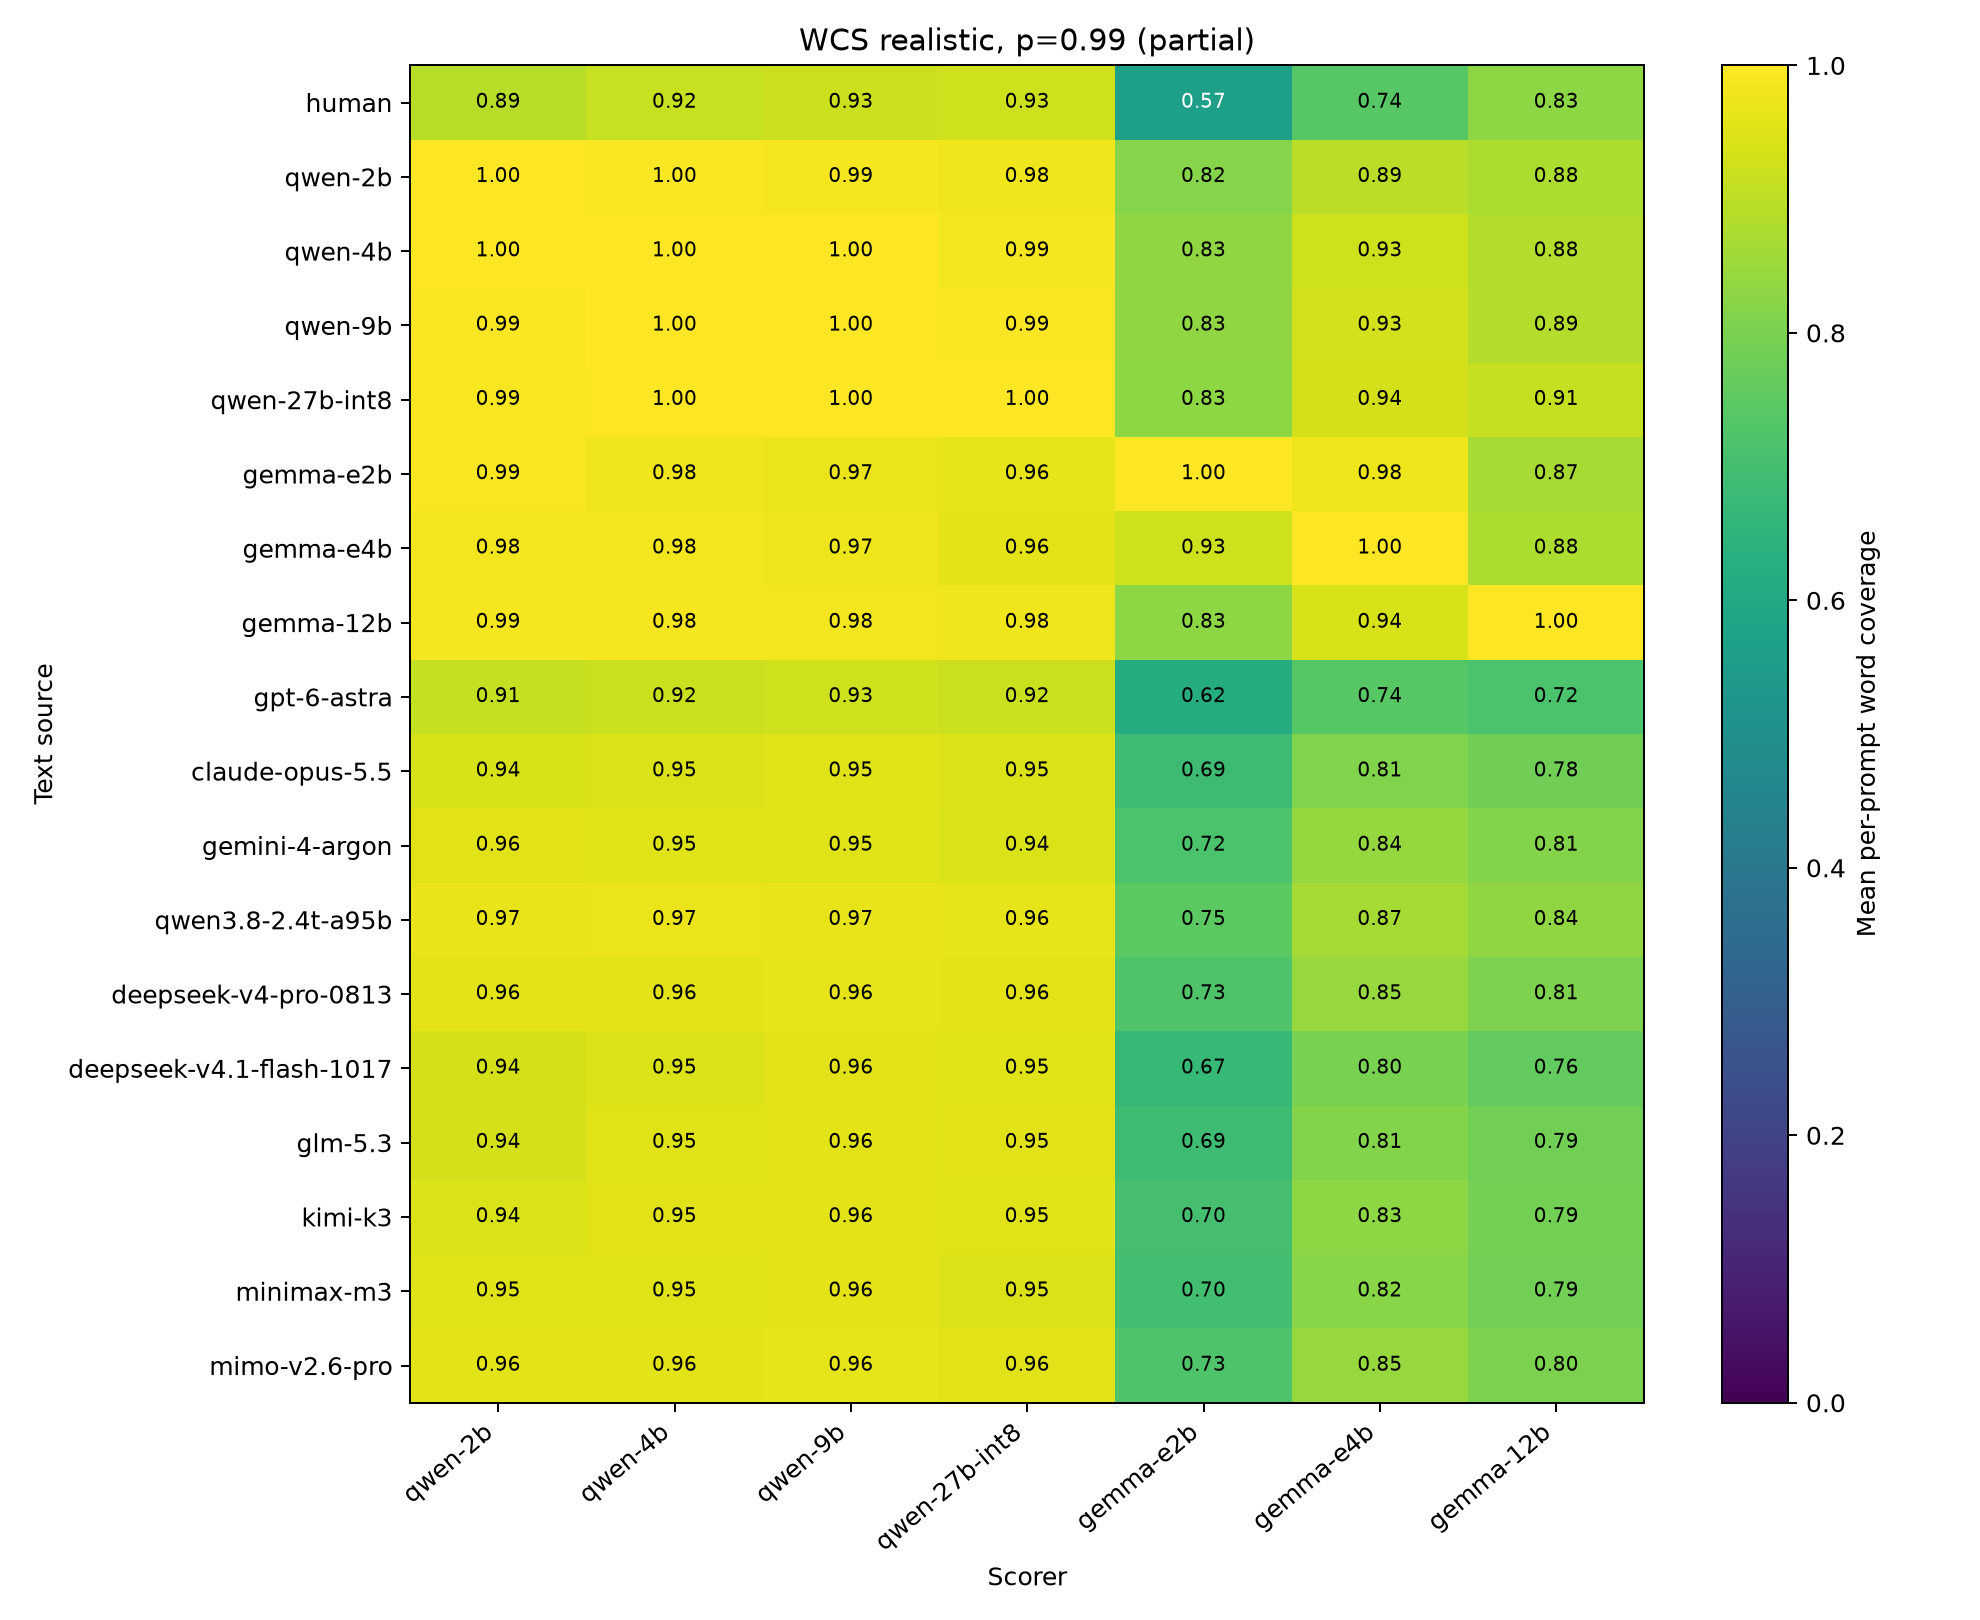
\includegraphics[width=0.94\textwidth]{figures/matrix-realistic-0.99.png}
\caption{\textbf{Empirical Scorer-by-Source Reachability Matrix} under realistic top-$p=0.99$ (top-$100$ normalized candidate pool) across 50 HC3 ELI5 prompts. Columns show open-weight scorers; rows show the 18 text sources spanning Human reference, Frontier Proprietary API models, Large Open-Weight frontier models ($427\text{B}$--$2.78\text{T}$), and Small Open-Weight local models ($\le 27\text{B}$).}
\label{fig:matrix}
\end{figure*}

In this paper, we use WCS to investigate a fundamental question about the contemporary LLM landscape: \emph{Why do frontier models appear so much closer to human writing than to small open-weight models when viewed through smaller scorers---and is this gap driven by weights access (closed vs.\ open), model scale, decoding temperature, or candidate-pool truncation?} To answer this question, we assemble a multi-tier, multi-domain, and multi-family experimental suite:
\begin{enumerate}
    \item \textbf{Three-Tier Source Stratification:} Beyond human answers and 7 small open-weight models ($\le 27\text{B}$), we collect and audit responses from \textbf{7 large open-weight frontier models} ($427\text{B}$--$2.78\text{T}$ parameters: Qwen3.8-2.4T-A95B, DeepSeek-V4-Pro, DeepSeek-V4.1-Flash, GLM-5.3, Kimi-K3, MiniMax-M3, MiMo-V2.6-Pro) alongside \textbf{3 proprietary frontier models} (GPT-6 Astra, Claude Opus 5.5, Gemini 4 Argon). This cleanly separates the effect of \emph{scale} within open-weight models from \emph{proprietary post-training}.
    \item \textbf{Scorer-Default \& Nucleus Filter Audits:} In addition to standardized realistic top-$p \in \{0.90, 0.95, 0.99\}$ filters, we evaluate reachability under each scorer's actual shipped \texttt{generation\_config.json} filter (\texttt{shipped}), non-thinking model-card defaults (\texttt{card\_nonthinking}), and unscaled $T=1.0$ filters (\texttt{unscaled\_T1}).
    \item \textbf{Exact Tail-Mass \& Top-1000 Validation:} We decompose the difference between top-$K$ renormalized nuclei (\texttt{realistic}) and exact full-vocabulary nuclei (\texttt{strict\_full}), running a dedicated GPU validation at $K=1000$ to quantify excluded tail mass $1 - M_K$.
    \item \textbf{Four-Family Scorer Pool \& Second-Domain Replication:} We expand the scorer pool from Qwen~3.5 and Gemma~4 to include \textbf{Llama-3.2-1B-Instruct}, \textbf{Llama-3.1-8B-Instruct} \cite{grattafiori2024llama3}, and \textbf{Mistral-7B-Instruct-v0.3} \cite{jiang2023mistral}, and replicate the full 3-tier audit on \textbf{HC3 Wikipedia CS/AI} (50 prompts).
\end{enumerate}

\section{Methodology}

\subsection{Word Coverage Score (WCS)}
Let $\mathcal{Q}$ be a benchmark of prompts, $\mathcal{S}$ a set of open-weight scoring models, and $\mathcal{G}$ a set of text sources. For prompt $q \in \mathcal{Q}$ and source $g \in \mathcal{G}$, let the response text $g(q)$ be segmented into $M$ whitespace-delimited words $(w_1, \dots, w_M)$ with character spans $\{[a_m, b_m)\}_{m=1}^M$.

When scorer $s \in \mathcal{S}$ processes the chat-formatted prompt prefix followed by $g(q)$, its tokenizer produces answer tokens $(t_1, \dots, t_N)$ with character offsets $\{[c_i, d_i)\}_{i=1}^N$. At each answer token position $i$, teacher forcing yields a conditional distribution $P_i = \mathbb{P}_s(\cdot \mid \text{prefix}, t_{<i})$ over the scorer's vocabulary $\mathcal{V}_s$. A candidate-pool filter $\mathcal{F}$ maps $P_i$ to a surviving candidate set $\mathcal{C}_{\mathcal{F}}(P_i) \subseteq \mathcal{V}_s$.

To prevent subword splitting from artificially inflating coverage on rare or compound words, we enforce the \textbf{all-subtoken survival rule}: word $w_m$ is covered if and only if every token $t_i$ whose character span overlaps $[a_m, b_m)$ satisfies $t_i \in \mathcal{C}_{\mathcal{F}}(P_i)$:
\begin{equation}
\text{cov}_{s,g}^{\mathcal{F}}(w_m) = \prod_{i:\, [c_i, d_i) \cap [a_m, b_m) \neq \emptyset} \mathbb{I}\!\left[t_i \in \mathcal{C}_{\mathcal{F}}(P_i)\right].
\end{equation}
The prompt-level score is $\text{WCS}_{s,g}^{\mathcal{F}}(q) = \frac{1}{M}\sum_{m=1}^M \text{cov}_{s,g}^{\mathcal{F}}(w_m)$, and the matrix cell is the prompt mean $\overline{\text{WCS}}_{s,g}^{\mathcal{F}} = \frac{1}{|\mathcal{Q}|}\sum_{q \in \mathcal{Q}} \text{WCS}_{s,g}^{\mathcal{F}}(q)$.

\subsection{Candidate-Pool Filter Families}
We evaluate four mathematically distinct candidate-pool filter families:
\begin{enumerate}
    \item \textbf{Realistic Top-$p$ over Top-$K$ (\texttt{realistic}):} Retains the top-$K$ ($K=100$ baseline, $K=1000$ in validation) highest-probability tokens at $T=1.0$, renormalizes their probabilities by $M_K = \sum_{r=1}^K P_i(v_{(r)})$, and includes tokens in descending rank order until cumulative renormalized mass reaches $p \in \{0.90, 0.95, 0.99\}$ (always including the first token that crosses $p$).
    \item \textbf{Strict Unnormalized Top-$K$ (\texttt{strict}):} Identical to \texttt{realistic} except cumulative mass is compared against $p$ without dividing by $M_K$.
    \item \textbf{Exact Full-Vocabulary Top-$p$ (\texttt{strict\_full}):} Evaluates survival over the complete vocabulary $\mathcal{V}_s$ without top-$K$ truncation: token $t_i$ survives iff the total probability mass of tokens strictly more probable than $t_i$ is less than $p$, i.e., $\sum_{v \in \mathcal{V}_s:\, P_i(v) > P_i(t_i)} P_i(v) < p$.
    \item \textbf{Scorer-Default Filter (\texttt{scorer\_default}):} Applies each scorer's native inference configuration $(T_s, k_s, p_s)$: logits are scaled by $1/T_s$, truncated to the top-$k_s$ candidates, renormalized, and filtered by nucleus threshold $p_s$. We audit three variants: (a) \texttt{shipped} (exact \texttt{generation\_config.json} defaults: $T=0.6, k=20, p=0.95$ for Qwen~3.5; $T=1.0, k=64, p=0.95$ for Gemma~4), (b) \texttt{card\_nonthinking} ($T=0.7, k=20, p=0.80$ for Qwen~3.5 non-thinking mode), and (c) \texttt{unscaled\_T1} (shipped $k_s, p_s$ at $T=1.0$).
\end{enumerate}

\subsection{Prompt-Paired Bootstrap Inference}
Because lexical difficulty varies substantially across questions, all source and tier comparisons are computed as prompt-paired differences. For any two sources (or tier averages) $A$ and $B$ evaluated across a common scorer set $\mathcal{S}^*$:
\begin{equation}
\Delta_{A - B}(q) = \frac{1}{|\mathcal{S}^*|} \sum_{s \in \mathcal{S}^*} \left(\text{WCS}_{s,A}(q) - \text{WCS}_{s,B}(q)\right).
\end{equation}
We report the prompt mean $\overline{\Delta}_{A - B}$ and $95\%$ percentile confidence intervals from $10,000$ paired bootstrap resamples over prompts (seed 42).

\begin{table*}[t]
\centering
\scriptsize
\setlength{\tabcolsep}{3.8pt}
\begin{tabular}{llcccccccc}
\toprule
\textbf{Tier} & \textbf{Source Generator} & \textbf{Qwen-2B} & \textbf{Qwen-4B} & \textbf{Qwen-9B} & \textbf{Qwen-27B*} & \textbf{Gem-E2B} & \textbf{Gem-E4B} & \textbf{Gem-12B} & \textbf{$\Delta_{\text{Human}-\text{Src}}$ (6-sc)} \\
\midrule
\textit{Human} & \textbf{Human (HC3 ELI5)} & 0.8930 & 0.9161 & 0.9250 & 0.9265 & 0.5660 & 0.7386 & 0.8288 & --- \\
\midrule
\multirow{3}{*}{\textit{Frontier Prop.}}
 & \textbf{GPT-6 Astra} & 0.9121 & 0.9194 & 0.9279 & 0.9186 & 0.6195 & 0.7392 & \textbf{0.7154} & \textbf{+0.0056} $[-0.0036, +0.0147]$ \\
 & \textbf{Claude Opus 5.5} & 0.9408 & 0.9455 & 0.9529 & 0.9479 & 0.6851 & 0.8106 & \textbf{0.7824} & $-0.0416$ $[-0.0499, -0.0335]$ \\
 & \textbf{Gemini 4 Argon} & 0.9555 & 0.9523 & 0.9509 & 0.9414 & 0.7175 & 0.8428 & \textbf{0.8128} & $-0.0607$ $[-0.0700, -0.0516]$ \\
\midrule
\multirow{7}{*}{\textit{Large Open-Wt.}}
 & \textbf{DeepSeek-V4.1-Flash} & 0.9363 & 0.9486 & 0.9552 & 0.9517 & 0.6683 & 0.7976 & \textbf{0.7578} & $-0.0327$ $[-0.0429, -0.0229]$ \\
 & \textbf{GLM-5.3} & 0.9362 & 0.9494 & 0.9574 & 0.9547 & 0.6888 & 0.8138 & \textbf{0.7864} & $-0.0441$ $[-0.0537, -0.0345]$ \\
 & \textbf{MiniMax-M3} & 0.9512 & 0.9530 & 0.9602 & 0.9469 & 0.6981 & 0.8242 & \textbf{0.7854} & $-0.0508$ $[-0.0599, -0.0419]$ \\
 & \textbf{Kimi-K3} & 0.9428 & 0.9532 & 0.9591 & 0.9527 & 0.7044 & 0.8286 & \textbf{0.7917} & $-0.0521$ $[-0.0624, -0.0413]$ \\
 & \textbf{MiMo-V2.6-Pro}$^{\dagger}$ & 0.9593 & 0.9602 & 0.9630 & 0.9568 & 0.7260 & 0.8467 & \textbf{0.8037} & $-0.0647$ $[-0.0741, -0.0554]$ \\
 & \textbf{DeepSeek-V4-Pro} & 0.9597 & 0.9606 & 0.9645 & 0.9574 & 0.7257 & 0.8462 & \textbf{0.8078} & $-0.0662$ $[-0.0774, -0.0553]$ \\
 & \textbf{Qwen3.8-2.4T-A95B} & 0.9651 & 0.9689 & 0.9687 & 0.9641 & 0.7469 & 0.8660 & 0.8354 & $-0.0806$ $[-0.0898, -0.0717]$ \\
\midrule
\multirow{7}{*}{\textit{Small Open-Wt.}}
 & \textbf{Qwen-2B}$^{\ddagger}$ & 1.0000 & 0.9955 & 0.9877 & 0.9780 & 0.8190 & 0.8950 & 0.8763 & $-0.1183$ $[-0.1286, -0.1086]$ \\
 & \textbf{Qwen-4B} & 0.9971 & 1.0000 & 0.9978 & 0.9867 & 0.8335 & 0.9283 & 0.8835 & $-0.1288$ $[-0.1382, -0.1197]$ \\
 & \textbf{Qwen-9B} & 0.9950 & 0.9987 & 1.0000 & 0.9932 & 0.8334 & 0.9313 & 0.8852 & $-0.1293$ $[-0.1390, -0.1198]$ \\
 & \textbf{Qwen-27B*} & 0.9910 & 0.9962 & 0.9973 & 1.0000 & 0.8306 & 0.9351 & 0.9112 & $-0.1323$ $[-0.1415, -0.1235]$ \\
 & \textbf{Gemma-12B} & 0.9855 & 0.9849 & 0.9817 & 0.9795 & 0.8286 & 0.9391 & 1.0000 & $-0.1420$ $[-0.1512, -0.1331]$ \\
 & \textbf{Gemma-E4B} & 0.9838 & 0.9809 & 0.9749 & 0.9607 & 0.9289 & 1.0000 & 0.8774 & $-0.1464$ $[-0.1554, -0.1378]$ \\
 & \textbf{Gemma-E2B} & 0.9884 & 0.9793 & 0.9721 & 0.9620 & 1.0000 & 0.9762 & 0.8691 & $-0.1529$ $[-0.1623, -0.1438]$ \\
\bottomrule
\end{tabular}
\caption{\textbf{Complete Realistic Top-$p=0.99$ WCS Matrix on HC3 ELI5.} Columns show the 7 open-weight scorers; rows show the 18 sources stratified by tier. Last column reports prompt-paired $\Delta_{\text{Human}-\text{Src}}$ and $95\%$ bootstrap CI across the 6 bf16 scorers with complete 18-source coverage ($N=50$ prompts; $^{\dagger}N=49$ for MiMo-V2.6-Pro; $^{\ddagger}N=48$ for Qwen-2B). Bold cells under Gemma-12B indicate machine sources that are \emph{less} reachable than human writing ($0.8288$).}
\label{tab:matrix_099}
\end{table*}

\section{Experimental Setup}

\paragraph{Benchmarks \& Prompt Selection:}
We evaluate two domains from the Human ChatGPT Comparison Corpus (HC3; pinned revision \texttt{4d0ff1873389...}) \cite{guo2023hc3} using deterministic reservoir sampling (seed 42) restricted to prompts whose curated human answer contains between 150 and 400 whitespace words:
\begin{enumerate}
    \item \textbf{HC3 Reddit ELI5} ($|\mathcal{Q}|=50$): Conversational explanatory questions; human answers average $234.6$ words (range $151$--$397$).
    \item \textbf{HC3 Wikipedia CS/AI (\texttt{wiki\_csai})} ($|\mathcal{Q}|=50$): Encyclopedic computer science and AI questions; human answers average $221.3$ words (range $151$--$386$).
\end{enumerate}

\paragraph{Source Tiers ($\mathcal{G}$, 18 Sources):}
All machine sources receive the exact same prompt question and length instruction (\emph{``Answer the following question in 150--400 words''}):
\begin{itemize}
    \item \textbf{Small Open-Weight Tier ($\le 32\text{B}$):} Qwen3.5-2B, Qwen3.5-4B, Qwen3.5-9B (bf16), Qwen3.5-27B (int8) \cite{qwen2026}, Gemma-4-E2B-it ($5.1\text{B}$), Gemma-4-E4B-it ($8.0\text{B}$), and Gemma-4-12B-it (bf16) \cite{gemma2026}. In our expanded 4-family experiment, we also generate from Llama-3.2-1B-Instruct, Llama-3.1-8B-Instruct, and Mistral-7B-Instruct-v0.3. Baseline local generation uses greedy decoding ($T=0$); our decoding ablation regenerates all 6 bf16 Qwen/Gemma models under stochastic sampling ($T=0.7, p=0.95, k=50$).
    \item \textbf{Large Open-Weight Tier ($427\text{B}$--$2.78\text{T}$):} Seven frontier-scale open-weight models accessed via OpenRouter with provenance preserved as \texttt{weights\_access: open\_weights}: \textbf{Qwen3.8-2.4T-A95B} ($2{,}400\text{B}$ total / $95\text{B}$ active), \textbf{DeepSeek-V4-Pro} ($951\text{B}$ total / $43\text{B}$ active), \textbf{DeepSeek-V4.1-Flash} ($427\text{B}$ total / $20\text{B}$ active), \textbf{GLM-5.3} ($1{,}120\text{B}$ total / $48\text{B}$ active), \textbf{Kimi-K3} ($1{,}500\text{B}$ total / $60\text{B}$ active), \textbf{MiniMax-M3} ($2{,}780\text{B}$ total / $85\text{B}$ active), and \textbf{MiMo-V2.6-Pro} ($457\text{B}$ total / $32\text{B}$ active). All 50 prompts are complete across all models except a single empty upstream response on prompt \texttt{eli5\_537} for MiMo-V2.6-Pro ($49/50$); we never impute missing cells and report both all-available ($N=50/49$) and strict complete-case ($N=49$) analyses.
    \item \textbf{Frontier Proprietary Tier:} \textbf{GPT-6 Astra} (\texttt{gpt-6-astra-2026-09-23}), \textbf{Claude Opus 5.5} (\texttt{claude-opus-5-5-20261001}), and \textbf{Gemini 4 Argon} (\texttt{gemini-4-argon-2026-09-29}), with 50/50 complete responses in both domains.
\end{itemize}

\paragraph{Scorer Pool ($\mathcal{S}$, 9 Open-Weight Scorers Across 4 Families):}
Our core comparison uses the 6 bf16 Qwen~3.5 and Gemma~4 scorers across all 18 sources (plus Qwen3.5-27B-int8 across all 18 sources). In Section~\ref{sec:expanded_scorers}, we add \textbf{Llama-3.2-1B-Instruct} ($1.24\text{B}$), \textbf{Llama-3.1-8B-Instruct} ($8.03\text{B}$), and \textbf{Mistral-7B-Instruct-v0.3} ($7.25\text{B}$) in bf16, yielding 9 bf16 scorers across 4 distinct model families and tokenizers. Teacher-forced audits run in 128-token KV-cached chunks with zero sequence truncation.

\begin{table*}[t]
\centering
\scriptsize
\setlength{\tabcolsep}{3.8pt}
\begin{tabular}{llcccccccc}
\toprule
\textbf{Tier} & \textbf{Source Generator} & \textbf{Qwen-2B} & \textbf{Qwen-4B} & \textbf{Qwen-9B} & \textbf{Qwen-27B*} & \textbf{Gem-E2B} & \textbf{Gem-E4B} & \textbf{Gem-12B} & \textbf{Shipped Default (6-sc)} \\
\midrule
\textit{Human} & \textbf{Human (HC3 ELI5)} & 0.8377 & 0.8622 & 0.8737 & 0.8659 & 0.4699 & 0.6316 & 0.7330 & 0.6448 \\
\midrule
\multirow{3}{*}{\textit{Frontier Prop.}}
 & \textbf{GPT-6 Astra} & 0.8263 & 0.8358 & 0.8490 & 0.8395 & 0.5165 & 0.6244 & 0.6054 & 0.6196 ($+0.0252$) \\
 & \textbf{Claude Opus 5.5} & 0.8717 & 0.8760 & 0.8877 & 0.8857 & 0.5843 & 0.7111 & 0.6849 & 0.6903 ($-0.0455$) \\
 & \textbf{Gemini 4 Argon} & 0.8914 & 0.8844 & 0.8814 & 0.8748 & 0.6293 & 0.7458 & 0.7266 & 0.7188 ($-0.0740$) \\
\midrule
\multirow{7}{*}{\textit{Large Open-Wt.}}
 & \textbf{DeepSeek-V4.1-Flash} & 0.8639 & 0.8801 & 0.8886 & 0.8860 & 0.5657 & 0.6894 & 0.6478 & 0.6746 ($-0.0299$) \\
 & \textbf{GLM-5.3} & 0.8680 & 0.8855 & 0.8956 & 0.8920 & 0.5930 & 0.7117 & 0.6836 & 0.6915 ($-0.0468$) \\
 & \textbf{MiniMax-M3} & 0.8894 & 0.8840 & 0.8954 & 0.8846 & 0.6039 & 0.7247 & 0.6843 & 0.7024 ($-0.0576$) \\
 & \textbf{Kimi-K3} & 0.8739 & 0.8869 & 0.8985 & 0.8945 & 0.6080 & 0.7292 & 0.6971 & 0.7037 ($-0.0589$) \\
 & \textbf{MiMo-V2.6-Pro}$^{\dagger}$ & 0.8984 & 0.8980 & 0.9028 & 0.8972 & 0.6280 & 0.7482 & 0.7112 & 0.7231 ($-0.0773$) \\
 & \textbf{DeepSeek-V4-Pro} & 0.8985 & 0.8980 & 0.9081 & 0.9030 & 0.6294 & 0.7474 & 0.7134 & 0.7282 ($-0.0834$) \\
 & \textbf{Qwen3.8-2.4T-A95B} & 0.9130 & 0.9151 & 0.9191 & 0.9167 & 0.6530 & 0.7743 & 0.7429 & 0.7517 ($-0.1069$) \\
\midrule
\multirow{7}{*}{\textit{Small Open-Wt.}}
 & \textbf{Qwen-2B}$^{\ddagger}$ & 1.0000 & 0.9783 & 0.9501 & 0.9312 & 0.7184 & 0.7997 & 0.7784 & 0.8386 ($-0.1949$) \\
 & \textbf{Qwen-4B} & 0.9840 & 1.0000 & 0.9850 & 0.9518 & 0.7426 & 0.8490 & 0.7956 & 0.8680 ($-0.2232$) \\
 & \textbf{Qwen-9B} & 0.9773 & 0.9897 & 1.0000 & 0.9689 & 0.7438 & 0.8524 & 0.8009 & 0.8673 ($-0.2225$) \\
 & \textbf{Qwen-27B*} & 0.9683 & 0.9800 & 0.9843 & 1.0000 & 0.7456 & 0.8611 & 0.8346 & 0.8556 ($-0.2108$) \\
 & \textbf{Gemma-12B} & 0.9555 & 0.9490 & 0.9409 & 0.9367 & 0.7408 & 0.8629 & 1.0000 & 0.8513 ($-0.2065$) \\
 & \textbf{Gemma-E4B} & 0.9526 & 0.9392 & 0.9262 & 0.9048 & 0.8566 & 1.0000 & 0.7888 & 0.8507 ($-0.2059$) \\
 & \textbf{Gemma-E2B} & 0.9629 & 0.9353 & 0.9205 & 0.9030 & 1.0000 & 0.9268 & 0.7768 & 0.8594 ($-0.2146$) \\
\bottomrule
\end{tabular}
\caption{\textbf{Realistic Top-$p=0.95$ WCS Matrix and Shipped Scorer-Default Summary on HC3 ELI5.} Columns 3--9 show cell means under realistic $p=0.95$; the final column shows the 6-scorer mean WCS (and paired $\Delta_{\text{Human}-\text{Src}}$) under each scorer's shipped \texttt{generation\_config.json} filter ($T=0.6, k=20, p=0.95$ for Qwen~3.5; $T=1.0, k=64, p=0.95$ for Gemma~4).}
\label{tab:matrix_095}
\end{table*}

\section{Empirical Results}

\subsection{The Three-Tier Reachability Hierarchy}
Tables~\ref{tab:matrix_099} and \ref{tab:matrix_095} report the complete scorer-by-source matrices on HC3 ELI5 at $p=0.99$ and $p=0.95$, and Table~\ref{tab:tier_contrasts} summarizes the prompt-paired tier contrasts across all filter conditions and domains.

Across the 6 complete bf16 scorers on HC3 ELI5 under \texttt{realistic} $p=0.99$:
\begin{itemize}
    \item \textbf{Human writing} has a mean WCS of \textbf{$0.8112$} ($0.8118$ on the 49 complete-case prompts).
    \item \textbf{Frontier Proprietary} models average \textbf{$0.8435$} ($\Delta_{\text{Human}-\text{Tier}} = -0.0322$, $95\%$ CI $[-0.0405, -0.0240]$). Within this tier, \textbf{GPT-6 Astra} ($\text{WCS}=0.8056$) is slightly \emph{less} reachable than human writing ($\Delta = +0.0056$, CI $[-0.0036, +0.0147]$), followed by Claude Opus 5.5 ($0.8529$, $\Delta = -0.0416$) and Gemini 4 Argon ($0.8720$, $\Delta = -0.0607$).
    \item \textbf{Large Open-Weight} frontier models ($427\text{B}$--$2.78\text{T}$) occupy a distinct middle tier with mean WCS of \textbf{$0.8672$} ($\Delta_{\text{Human}-\text{Tier}} = -0.0555$, CI $[-0.0644, -0.0467]$). Every individual large open-weight model falls between the small open-weight tier and human writing: DeepSeek-V4.1-Flash ($0.8440$, $\Delta = -0.0327$), GLM-5.3 ($0.8553$, $\Delta = -0.0441$), MiniMax-M3 ($0.8620$, $\Delta = -0.0508$), Kimi-K3 ($0.8633$, $\Delta = -0.0521$), MiMo-V2.6-Pro ($0.8765$, $\Delta = -0.0647$), DeepSeek-V4-Pro ($0.8774$, $\Delta = -0.0662$), and Qwen3.8-2.4T-A95B ($0.8919$, $\Delta = -0.0806$).
    \item \textbf{Small Open-Weight} local models ($\le 27\text{B}$) are highly reachable across all scorers, averaging \textbf{$0.9466$} ($\Delta_{\text{Human}-\text{Tier}} = -0.1360$, CI $[-0.1455, -0.1270]$).
\end{itemize}

Crucially, the paired tier contrast between \textbf{Large Open-Weight and Small Open-Weight} is \textbf{$-0.0795$} ($95\%$ CI $[-0.0833, -0.0757]$), while the contrast between \textbf{Large Open-Weight and Frontier Proprietary} is \textbf{$+0.0234$} ($95\%$ CI $[+0.0207, +0.0263]$). This resolves a key ambiguity: \emph{more than three-quarters of the reachability gap between small local models and proprietary frontier models is already present when scaling up to $427\text{B}$--$2.78\text{T}$ open-weight models.} Under Gemma-12B ($\text{Human}=0.8288$), 9 of the 10 frontier-scale models (all 3 proprietary models and 6 of 7 large open-weight models, save Qwen3.8-2.4T at $0.8354$) fall \emph{below} human coverage.

\paragraph{Length-Matched Prefix Sensitivity Check:}
Because frontier responses are slightly longer on average ($262$--$365$ words vs.\ $235$ for human), we recompute WCS restricted to the first 150 whitespace words of every response (\texttt{prefix150} in Table~\ref{tab:source_deltas}). The three-tier ordering is completely unchanged: $\Delta_{\text{Human}-\text{Src}}$ is $-0.0083$ for GPT-6 Astra, $-0.0458$ for Claude Opus 5.5, $-0.0420$ to $-0.0871$ for Large Open-Weight models, and $-0.1258$ to $-0.1670$ for Small Open-Weight models.

\subsection{Scorer-Default Filter Audit}
Real deployments do not sample from $T=1.0$ top-$100$ pools; they use model-specific \texttt{generation\_config.json} filters. As shown in Table~\ref{tab:matrix_095} (last column) and Table~\ref{tab:tier_contrasts} (\texttt{default\_shipped}), evaluating under each scorer's shipped filter ($T=0.6, k=20, p=0.95$ for Qwen~3.5; $T=1.0, k=64, p=0.95$ for Gemma~4) sharpens the separation between tiers:
\begin{itemize}
    \item Human reachability drops to $0.6448$, while Small Open-Weight reachability remains high at $0.8553$ ($\Delta = -0.2116$, CI $[-0.2260, -0.1982]$).
    \item Large Open-Weight models drop to $0.7109$ ($\text{Large OW} - \text{Small OW} = -0.1450$, CI $[-0.1518, -0.1381]$).
    \item Frontier Proprietary models drop to $0.6762$ ($\Delta = -0.0314$), with GPT-6 Astra ($0.6196$) significantly \emph{less} reachable than human writing ($\Delta = +0.0252$, $95\%$ CI $[+0.0101, +0.0400]$).
\end{itemize}
Under Qwen~3.5's stricter non-thinking model-card defaults ($T=0.7, k=20, p=0.80$; \texttt{default\_card\_nonthinking}), the tier contrasts widen even further ($\text{Large OW} - \text{Small OW} = -0.1539$), while removing Qwen's temperature scaling (\texttt{default\_unscaled\_T1}, $T=1.0, k=20, p=0.95$) still yields $\text{Large OW} - \text{Small OW} = -0.1218$. Thus, narrow top-$k$ candidate pools ($k \in \{20, 64\}$) penalize both human and frontier writing far more severely than small open-weight text.

\begin{table*}[t]
\centering
\scriptsize
\setlength{\tabcolsep}{4.2pt}
\begin{tabular}{llcccccc}
\toprule
\textbf{Tier} & \textbf{Source} & \textbf{Realistic $0.99$} & \textbf{Realistic $0.95$} & \textbf{Realistic $0.90$} & \textbf{Strict-Full $0.99$} & \textbf{Shipped Default} & \textbf{Prefix-150 ($0.99$)} \\
\midrule
\multirow{3}{*}{\textit{Frontier Prop.}}
 & GPT-6 Astra & $+0.0056$ & $+0.0251$ & $+0.0298$ & \textbf{+0.0297} & $+0.0252$ & $-0.0083$ \\
 & Claude Opus 5.5 & $-0.0416$ & $-0.0346$ & $-0.0342$ & $-0.0122$ & $-0.0455$ & $-0.0458$ \\
 & Gemini 4 Argon & $-0.0607$ & $-0.0585$ & $-0.0609$ & $-0.0284$ & $-0.0740$ & $-0.0734$ \\
\midrule
\multirow{7}{*}{\textit{Large Open-Wt.}}
 & DeepSeek-V4.1-Flash & $-0.0327$ & $-0.0212$ & $-0.0177$ & $-0.0033$ & $-0.0299$ & $-0.0420$ \\
 & GLM-5.3 & $-0.0441$ & $-0.0382$ & $-0.0367$ & $-0.0151$ & $-0.0468$ & $-0.0520$ \\
 & MiniMax-M3 & $-0.0508$ & $-0.0456$ & $-0.0457$ & $-0.0195$ & $-0.0576$ & $-0.0588$ \\
 & Kimi-K3 & $-0.0521$ & $-0.0476$ & $-0.0479$ & $-0.0208$ & $-0.0589$ & $-0.0616$ \\
 & MiMo-V2.6-Pro & $-0.0647$ & $-0.0624$ & $-0.0634$ & $-0.0300$ & $-0.0773$ & $-0.0730$ \\
 & DeepSeek-V4-Pro & $-0.0662$ & $-0.0644$ & $-0.0657$ & $-0.0315$ & $-0.0834$ & $-0.0752$ \\
 & Qwen3.8-2.4T-A95B & $-0.0806$ & $-0.0849$ & $-0.0886$ & $-0.0453$ & $-0.1069$ & $-0.0871$ \\
\midrule
\multirow{7}{*}{\textit{Small Open-Wt.}}
 & Qwen-2B & $-0.1183$ & $-0.1370$ & $-0.1531$ & $-0.0789$ & $-0.1949$ & $-0.1258$ \\
 & Qwen-4B & $-0.1288$ & $-0.1580$ & $-0.1788$ & $-0.0888$ & $-0.2232$ & $-0.1397$ \\
 & Qwen-9B & $-0.1293$ & $-0.1593$ & $-0.1804$ & $-0.0893$ & $-0.2225$ & $-0.1424$ \\
 & Qwen-27B-int8 & $-0.1323$ & $-0.1610$ & $-0.1794$ & $-0.0927$ & $-0.2108$ & $-0.1474$ \\
 & Gemma-12B & $-0.1420$ & $-0.1735$ & $-0.1903$ & $-0.1038$ & $-0.2065$ & $-0.1539$ \\
 & Gemma-E4B & $-0.1464$ & $-0.1759$ & $-0.1932$ & $-0.1073$ & $-0.2059$ & $-0.1602$ \\
 & Gemma-E2B & $-0.1529$ & $-0.1857$ & $-0.2029$ & $-0.1140$ & $-0.2146$ & $-0.1670$ \\
\bottomrule
\end{tabular}
\caption{\textbf{Source-Level Paired Reachability Deltas ($\Delta_{\text{Human}-\text{Src}}$) Across Filter Regimes on HC3 ELI5} (averaged over the 6 complete bf16 scorers). Positive values indicate the source is \emph{less} reachable than human writing.}
\label{tab:source_deltas}
\end{table*}

\subsection{Decoding Ablation: Greedy ($T=0$) vs.\ Stochastic Sampling ($T>0$)}
Could small open-weight models appear more reachable simply because they were decoded greedily ($T=0$), whereas API frontier models use stochastic sampling? In our sampled-open-frontier experiment, we regenerate all 6 bf16 Qwen~3.5 and Gemma~4 sources at $T=0.7, \text{top\_p}=0.95, \text{top\_k}=50$.

As shown in Table~\ref{tab:tier_contrasts} (Sampled $T>0$ rows), stochastic sampling slightly reduces small open-weight reachability from $0.9466$ to $0.9357$ at $p=0.99$ ($\Delta_{\text{Human}-\text{Small OW}}$ shifts by $+0.0115$, from $-0.1360$ to $-0.1245$). However, a massive gap remains between sampled Small Open-Weight models ($0.9357$) and both Large Open-Weight ($0.8672$, paired contrast $-0.0684$, $95\%$ CI $[-0.0723, -0.0646]$) and Frontier Proprietary ($0.8435$, paired contrast $-0.0922$, CI $[-0.0963, -0.0882]$). At $p=0.95$, the contrast between Large Open-Weight and sampled Small Open-Weight is $-0.0945$ (CI $[-0.0996, -0.0896]$), and under \texttt{default\_shipped} it is $-0.1177$ (CI $[-0.1240, -0.1116]$). Thus, \textbf{decoding randomness accounts for less than $15\%$ of the reachability gap between small local models and frontier tiers.}

\begin{table*}[t]
\centering
\scriptsize
\resizebox{\textwidth}{!}{%
\begin{tabular}{llcccccc}
\toprule
\textbf{Experiment / Domain} & \textbf{Condition} & \textbf{Human} & \textbf{Frontier Prop.} & \textbf{Large OW} & \textbf{Small OW} & \textbf{Large OW $-$ Small OW} & \textbf{Large OW $-$ Frontier Prop.} \\
\midrule
\multirow{5}{*}{\textbf{ELI5 Core (6 bf16 sc.)}}
 & Realistic $p=0.99$ & 0.8112 & 0.8435 & 0.8672 & 0.9466 & $-0.0795$ $[-0.0833, -0.0757]$ & $+0.0234$ $[+0.0207, +0.0263]$ \\
 & Realistic $p=0.95$ & 0.7347 & 0.7573 & 0.7869 & 0.8985 & $-0.1119$ $[-0.1170, -0.1069]$ & $+0.0291$ $[+0.0259, +0.0326]$ \\
 & Realistic $p=0.90$ & 0.6822 & 0.7040 & 0.7347 & 0.8642 & $-0.1299$ $[-0.1357, -0.1241]$ & $+0.0302$ $[+0.0264, +0.0342]$ \\
 & Strict-Full $p=0.99$ & 0.8525 & 0.8562 & 0.8762 & 0.9485 & $-0.0725$ $[-0.0755, -0.0695]$ & $+0.0198$ $[+0.0173, +0.0224]$ \\
 & Shipped Default & 0.6448 & 0.6762 & 0.7109 & 0.8553 & $-0.1450$ $[-0.1518, -0.1381]$ & $+0.0341$ $[+0.0298, +0.0385]$ \\
\midrule
\multirow{3}{*}{\textbf{ELI5 Sampled $T>0$ (6 sc.)}}
 & Realistic $p=0.99$ & 0.8112 & 0.8435 & 0.8672 & 0.9357 & $-0.0684$ $[-0.0723, -0.0646]$ & $+0.0234$ $[+0.0207, +0.0263]$ \\
 & Realistic $p=0.95$ & 0.7347 & 0.7573 & 0.7869 & 0.8815 & $-0.0945$ $[-0.0996, -0.0896]$ & $+0.0291$ $[+0.0259, +0.0326]$ \\
 & Shipped Default & 0.6448 & 0.6762 & 0.7109 & 0.8286 & $-0.1177$ $[-0.1240, -0.1116]$ & $+0.0341$ $[+0.0298, +0.0385]$ \\
\midrule
\multirow{3}{*}{\textbf{ELI5 4-Family (9 bf16 sc.)}}
 & Realistic $p=0.99$ & 0.8357 & 0.8670 & 0.8859 & 0.9471 & $-0.0614$ $[-0.0649, -0.0579]$ & $+0.0185$ $[+0.0162, +0.0210]$ \\
 & Realistic $p=0.95$ & 0.7615 & 0.7873 & 0.8124 & 0.9016 & $-0.0894$ $[-0.0940, -0.0848]$ & $+0.0247$ $[+0.0218, +0.0277]$ \\
 & Strict-Full $p=0.99$ & \textbf{0.8794} & \textbf{0.8844} & 0.9001 & 0.9522 & $-0.0523$ $[-0.0552, -0.0494]$ & $+0.0155$ $[+0.0133, +0.0177]$ \\
\midrule
\multirow{4}{*}{\textbf{Wiki CS/AI (6 bf16 sc.)}}
 & Realistic $p=0.99$ & 0.8233 & 0.8638 & 0.8876 & 0.9501 & $-0.0625$ $[-0.0663, -0.0588]$ & $+0.0239$ $[+0.0210, +0.0267]$ \\
 & Realistic $p=0.95$ & 0.7463 & 0.7928 & 0.8200 & 0.9072 & $-0.0872$ $[-0.0919, -0.0825]$ & $+0.0273$ $[+0.0238, +0.0308]$ \\
 & Strict-Full $p=0.99$ & 0.8543 & 0.8719 & 0.8938 & 0.9519 & $-0.0581$ $[-0.0613, -0.0550]$ & $+0.0219$ $[+0.0195, +0.0244]$ \\
 & Shipped Default & 0.6584 & 0.7284 & 0.7595 & 0.8687 & $-0.1092$ $[-0.1157, -0.1028]$ & $+0.0311$ $[+0.0264, +0.0358]$ \\
\bottomrule
\end{tabular}%
}
\caption{\textbf{Tier-Level Means and Prompt-Paired Contrasts Across Experiments, Filter Regimes, and Domains.} All bracketed intervals are $95\%$ paired bootstrap CIs ($10{,}000$ replicates). Under 9-scorer Strict-Full $p=0.99$, Human ($0.8794$) and Frontier Proprietary ($0.8844$) have $\Delta = -0.0050$ ($95\%$ CI $[-0.0103, +0.0001]$, overlapping zero).}
\label{tab:tier_contrasts}
\end{table*}

\subsection{Top-100 vs.\ Top-1000 vs.\ Full-Vocabulary Nucleus Validation}
Why does human reachability increase more than machine reachability when moving from \texttt{realistic} (top-$100$ renormalized) to \texttt{strict\_full} (exact full-vocabulary nucleus)? When a scorer's distribution is high-entropy (flat), the top-$100$ candidates capture less than $p=0.99$ of the total probability mass ($M_{100} < 0.99$). Renormalizing by $M_{100}$ truncates valid tail tokens of rank $>100$ that would otherwise lie inside the true full-vocabulary $p=0.99$ nucleus.

To measure this mechanism directly, we ran a dedicated GPU validation auditing \textbf{Qwen-9B} and \textbf{Gemma-12B} at \textbf{$K=1000$} across all 18 sources and comparing against $K=100$ and exact $|\mathcal{V}_s|$ (Table~\ref{tab:top1000}):
\begin{enumerate}
    \item \textbf{Excluded Tail Mass ($1 - M_K$):} On human text, Qwen-9B places $2.67\%$ mean probability mass outside its top-$100$ candidates ($1 - M_{100} = 0.0267$), causing a $4.86\%$ top-$100$ miss rate and a $+0.0476$ gap between \texttt{strict\_full} ($0.9727$) and \texttt{realistic} ($0.9250$) at $p=0.99$. Expanding support to $K=1000$ reduces excluded tail mass $5.6\times$ to $0.48\%$ ($1 - M_{1000} = 0.0048$), raising \texttt{realistic} WCS to \textbf{$0.9644$} and closing \textbf{$82.7\%$} of the truncation gap. On Gemma-12B, expanding $K=100 \to 1000$ reduces human excluded tail mass nearly $10\times$ from $1.11\%$ to $0.12\%$, raising \texttt{realistic} WCS from $0.8288$ to \textbf{$0.8637$} (vs.\ $0.8712$ exact \texttt{strict\_full}, closing \textbf{$82.3\%$} of the gap).
    \item \textbf{Machine Sources Have Negligible Tail Mass Beyond Rank 1000:} On Qwen-9B and Gemma-12B, machine-generated texts place only $0.01\%$--$0.05\%$ mass outside top-$1000$ on Qwen-9B and $<0.003\%$ on Gemma-12B, so top-$1000$ \texttt{realistic} matches exact \texttt{strict\_full} within $0.0006$--$0.0020$ WCS across all machine tiers.
    \item \textbf{Full-Vocabulary Parity Between Human and Frontier Proprietary:} Under exact \texttt{strict\_full} $p=0.99$ across the 6 Qwen/Gemma scorers, the human--tier difference for Frontier Proprietary shrinks to $\Delta = -0.0036$ ($95\%$ CI $[-0.0100, +0.0025]$, statistically indistinguishable from zero!), while GPT-6 Astra ($0.8229$ vs.\ Human $0.8525$) is significantly \emph{less} reachable than human writing ($\Delta = +0.0297$, CI $[+0.0222, +0.0369]$). Even without top-$100$ support truncation, Large Open-Weight ($0.8762$) and Small Open-Weight ($0.9485$) remain cleanly separated ($\text{Large OW} - \text{Small OW} = -0.0725$, CI $[-0.0755, -0.0695]$).
\end{enumerate}

\begin{table*}[t]
\centering
\scriptsize
\setlength{\tabcolsep}{4.2pt}
\begin{tabular}{llccccccc}
\toprule
\textbf{Scorer} & \textbf{Source / Tier} & \textbf{$1 - M_{100}$} & \textbf{$1 - M_{1000}$} & \textbf{Top-100 Miss} & \textbf{Top-1000 Miss} & \textbf{WCS ($K=100$)} & \textbf{WCS ($K=1000$)} & \textbf{WCS (Full $|\mathcal{V}|$)} \\
\midrule
\multirow{5}{*}{\textbf{Qwen-9B}}
 & \textbf{Human (HC3)} & 2.672\% & 0.481\% & 4.858\% & 0.814\% & 0.9250 & \textbf{0.9644} & \textbf{0.9727} \\
 & \textbf{GPT-6 Astra} & 0.470\% & 0.054\% & 1.703\% & 0.098\% & 0.9279 & 0.9432 & 0.9451 \\
 & \textbf{Claude Opus 5.5} & 0.374\% & 0.048\% & 0.765\% & 0.033\% & 0.9529 & 0.9618 & 0.9633 \\
 & \textbf{Large Open-Wt.\ (mean)} & 0.311\% & 0.036\% & 0.693\% & 0.053\% & 0.9612 & 0.9672 & 0.9683 \\
 & \textbf{Small Open-Wt.\ (mean)} & 0.175\% & 0.020\% & 0.100\% & 0.001\% & 0.9869 & 0.9888 & 0.9890 \\
\midrule
\multirow{5}{*}{\textbf{Gemma-12B}}
 & \textbf{Human (HC3)} & 1.109\% & 0.117\% & 8.014\% & 2.054\% & 0.8288 & \textbf{0.8637} & \textbf{0.8712} \\
 & \textbf{GPT-6 Astra} & 0.046\% & 0.003\% & 3.662\% & 0.517\% & 0.7154 & 0.7210 & 0.7225 \\
 & \textbf{Claude Opus 5.5} & 0.026\% & 0.002\% & 1.516\% & 0.183\% & 0.7824 & 0.7845 & 0.7860 \\
 & \textbf{Large Open-Wt.\ (mean)} & 0.022\% & 0.001\% & 1.633\% & 0.208\% & 0.7954 & 0.7976 & 0.7990 \\
 & \textbf{Small Open-Wt.\ (mean)} & 0.013\% & 0.001\% & 0.268\% & 0.020\% & 0.9004 & 0.9012 & 0.9020 \\
\bottomrule
\end{tabular}
\caption{\textbf{Excluded Tail Mass ($1 - M_K$) and Candidate-Support Validation ($K=100$ vs.\ $K=1000$ vs.\ Full Vocabulary $|\mathcal{V}|$)} at $p=0.99$ on HC3 ELI5. Expanding candidate support from top-$100$ to top-$1000$ eliminates $>82\%$ of the support-truncation gap on human writing and makes human writing \emph{more} reachable than GPT-6 Astra on both Qwen-9B ($0.9644$ vs.\ $0.9432$) and Gemma-12B ($0.8637$ vs.\ $0.7210$).}
\label{tab:top1000}
\end{table*}

\begin{figure*}[t]
\centering
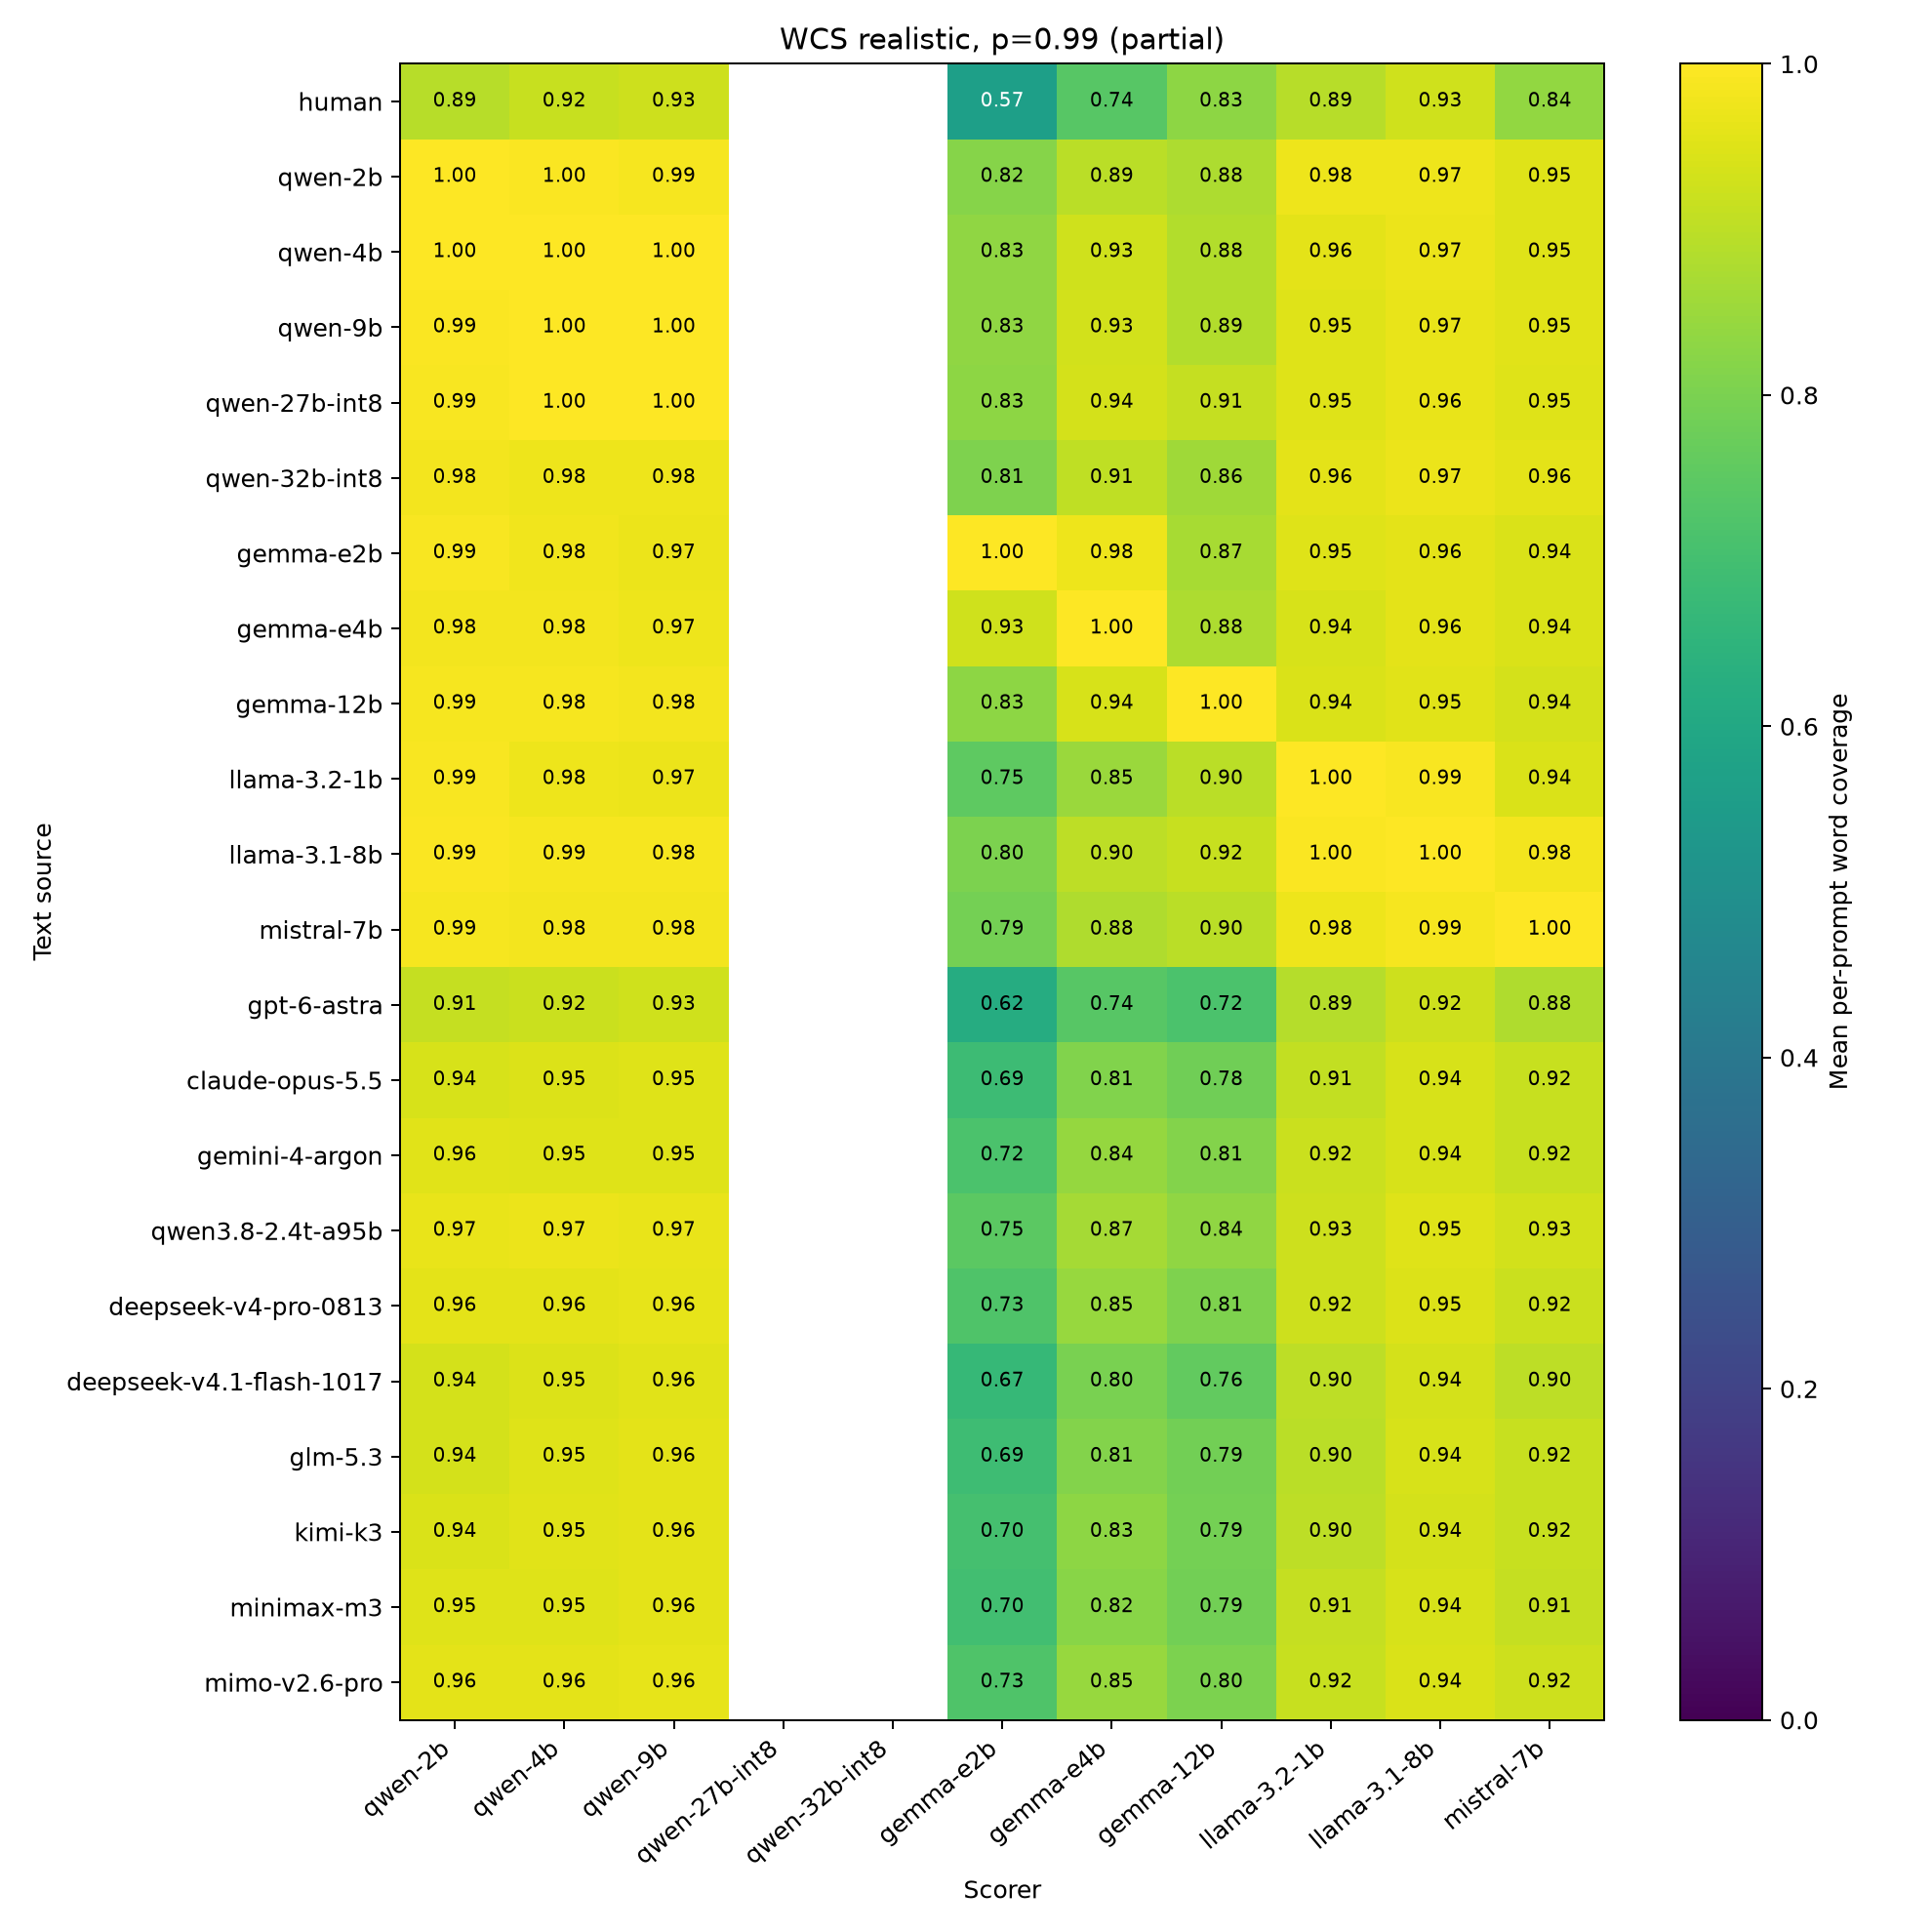
\includegraphics[width=0.49\textwidth]{figures/matrix-expanded-realistic-0.99.png}\hfill
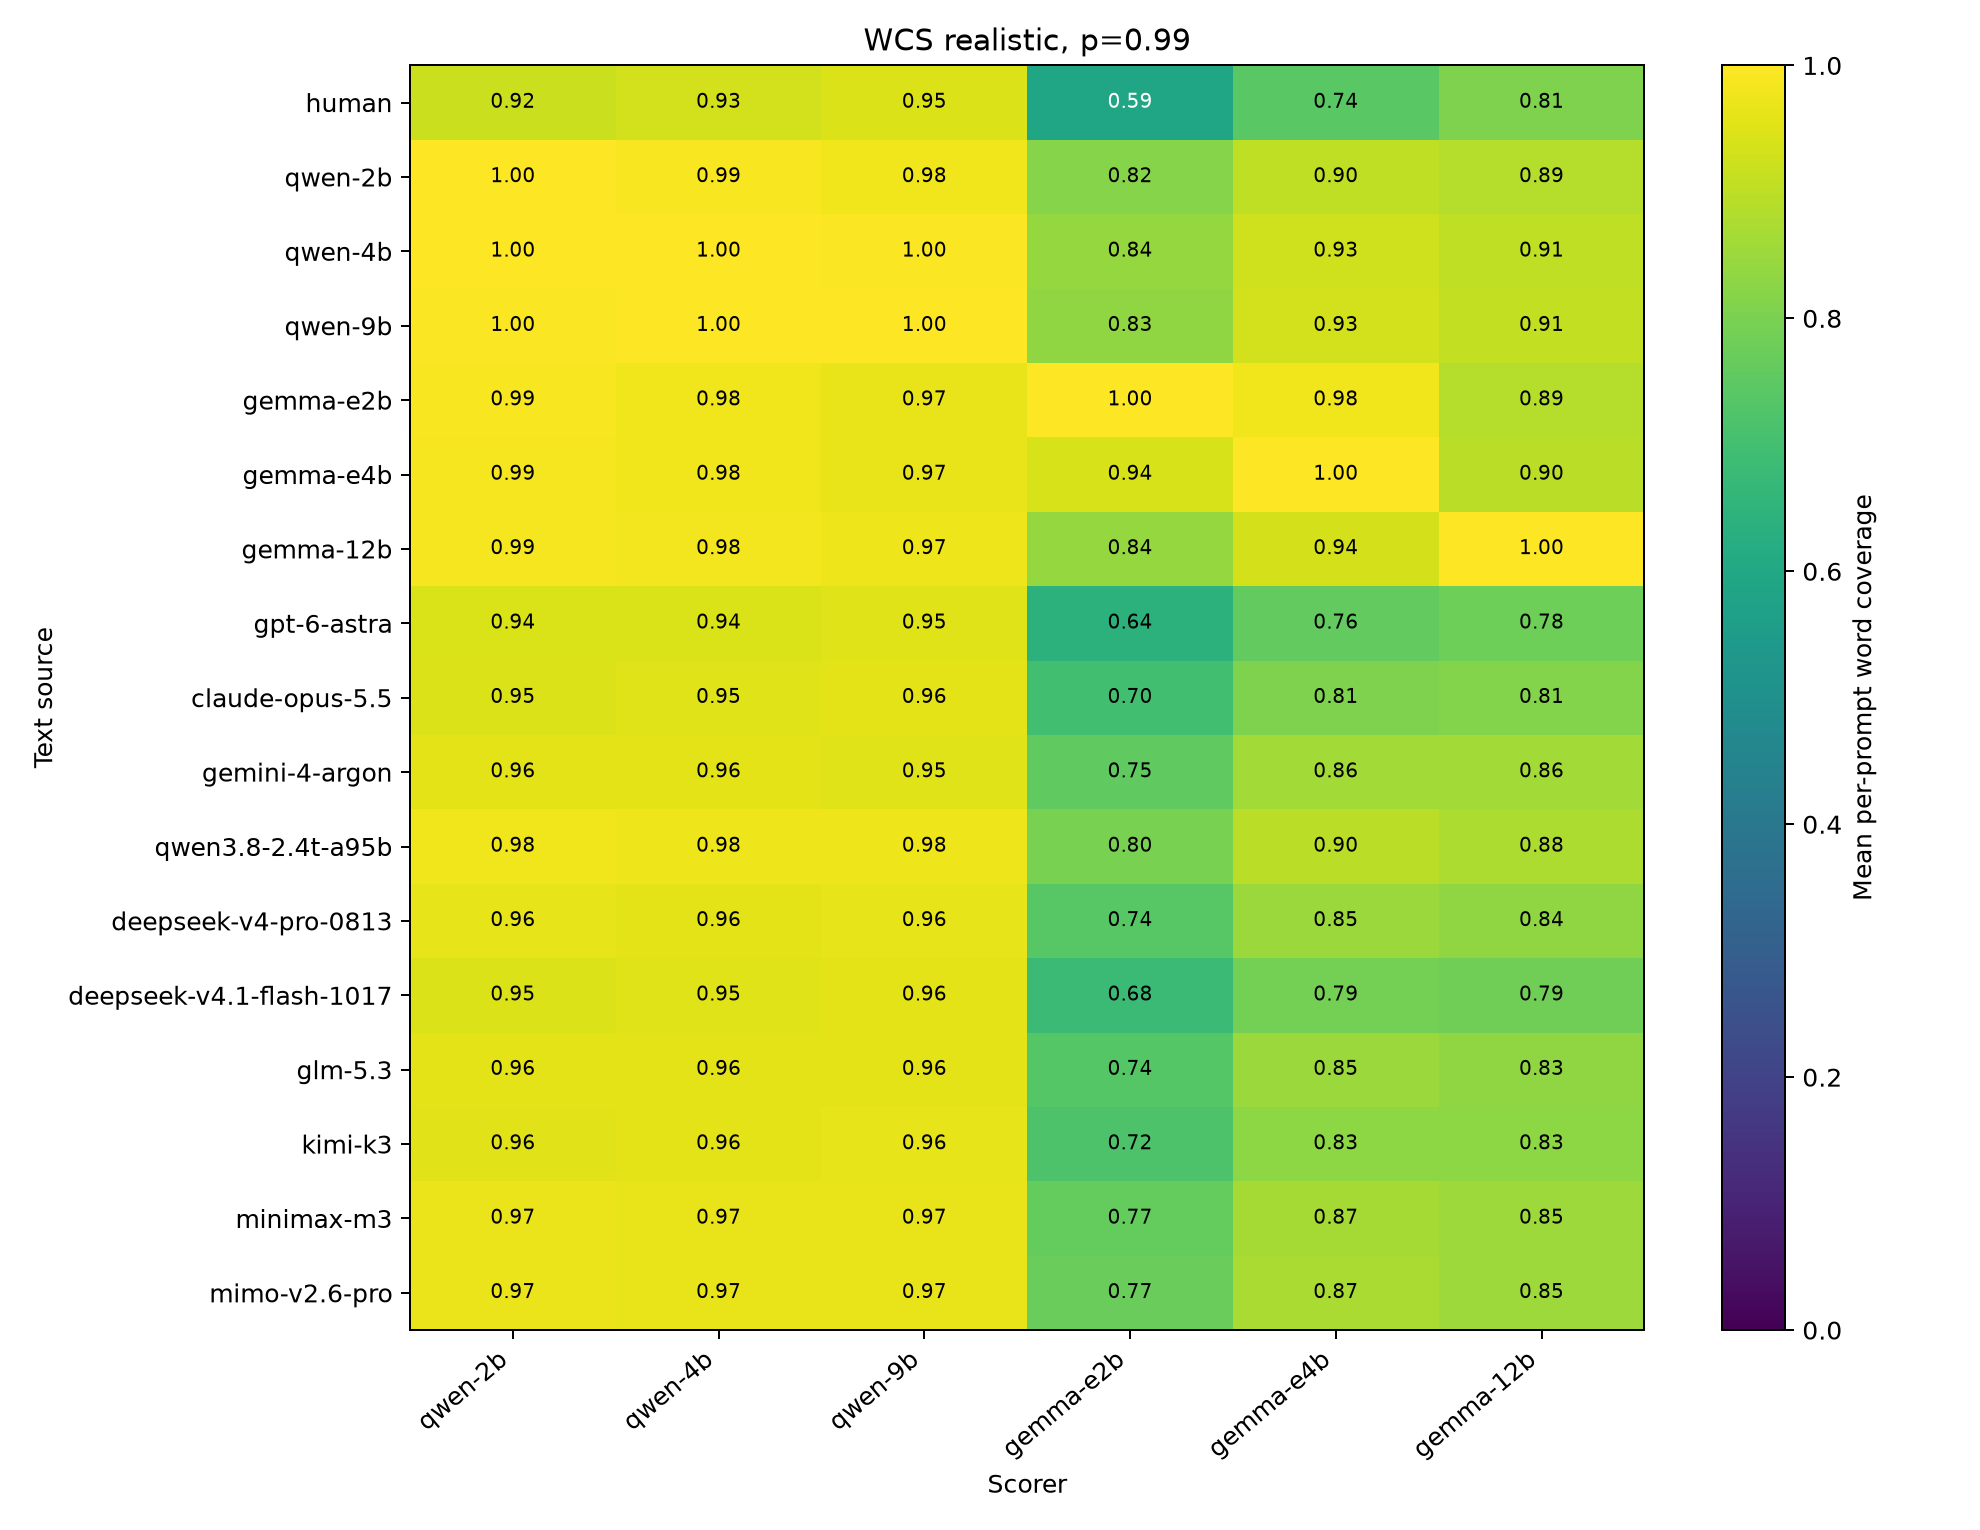
\includegraphics[width=0.49\textwidth]{figures/matrix-wiki-realistic-0.99.png}
\caption{\textbf{Cross-Family and Cross-Domain Generalization of the Reachability Matrix} (realistic top-$p=0.99$). \emph{Left:} 4-family expanded scorer pool (Qwen~3.5, Gemma~4, Llama~3.1/3.2, Mistral~7B; 9 bf16 scorers) on HC3 ELI5. \emph{Right:} Second-domain replication across all 16 sources on HC3 Wikipedia CS/AI (50 prompts).}
\label{fig:generalization}
\end{figure*}

\subsection{Generalization Across Four Scorer Families \& Second Domain}
\label{sec:expanded_scorers}

\paragraph{Four-Family Scorer Generalization (Qwen, Gemma, Llama, Mistral):}
To verify that our findings are not an artifact of Qwen~3.5 and Gemma~4's 256k-token vocabularies or training pipelines, we audited all 18 ELI5 sources (plus Llama-3.2-1B, Llama-3.1-8B, and Mistral-7B as sources) across \textbf{9 bf16 scorers spanning 4 families} (adding Llama-3.2-1B-Instruct, Llama-3.1-8B-Instruct, and Mistral-7B-Instruct-v0.3).
As shown in Table~\ref{tab:tier_contrasts} (\textbf{ELI5 4-Family}), the three-tier hierarchy holds across all 9 scorers:
\begin{itemize}
    \item Under \texttt{realistic} $p=0.99$: $\text{Human} = 0.8357$, $\text{Frontier Proprietary} = 0.8670$ ($\Delta = -0.0313$, CI $[-0.0388, -0.0238]$; GPT-6 Astra $= 0.8360$, $\Delta = -0.0002$), $\text{Large Open-Weight} = 0.8859$ ($\Delta = -0.0496$), and $\text{Small Open-Weight} = 0.9471$ ($\Delta = -0.1117$).
    \item Under \texttt{strict\_full} $p=0.99$ across all 9 scorers: $\text{Human} = 0.8794$ and $\text{Frontier Proprietary} = 0.8844$ ($\Delta = -0.0050$, $95\%$ CI $[-0.0103, +0.0001]$), whereas $\text{Large Open-Weight} = 0.9001$ and $\text{Small Open-Weight} = 0.9522$.
    \item \textbf{Same-Family Advantage:} Across Qwen and Gemma scorers/sources, same-family pairs exceed cross-family pairs (excluding self-coverage) by $\Delta_{\text{family}} = +0.0339$ at $p=0.99$ ($95\%$ CI $[+0.0322, +0.0355]$), $+0.0576$ at $p=0.95$, and $+0.0697$ at $p=0.90$. Across all 4 families ($14$ same-family vs.\ $64$ cross-family off-diagonal cells), the advantage remains highly significant at $+0.0156$ ($p=0.99$, CI $[+0.0137, +0.0176]$), $+0.0338$ ($p=0.95$), and $+0.0466$ ($p=0.90$).
\end{itemize}

\paragraph{Second-Domain Replication on Wikipedia CS/AI:}
Evaluating all 16 sources (Human, 6 Small Open-Weight, 7 Large Open-Weight, 3 Frontier Proprietary) across the 6 bf16 scorers on 50 formal encyclopedic \textbf{HC3 Wikipedia CS/AI} prompts (Table~\ref{tab:tier_contrasts}, \textbf{Wiki CS/AI}) replicates every structural property of the matrix:
\begin{itemize}
    \item At \texttt{realistic} $p=0.99$, reachability progresses monotonically across the four groups: \textbf{Human} ($0.8233$) $<$ \textbf{Frontier Proprietary} ($0.8638$, $\Delta = -0.0404$) $<$ \textbf{Large Open-Weight} ($0.8876$, $\Delta = -0.0643$) $<$ \textbf{Small Open-Weight} ($0.9501$, $\Delta = -0.1268$).
    \item Within Large Open-Weight on Wikipedia CS/AI, the model ordering closely mirrors ELI5: DeepSeek-V4.1-Flash ($0.8522$, $\Delta = -0.0289$), Kimi-K3 ($0.8761$), GLM-5.3 ($0.8828$), DeepSeek-V4-Pro ($0.8855$), MiniMax-M3 ($0.8981$), MiMo-V2.6-Pro ($0.9012$), and Qwen3.8-2.4T-A95B ($0.9173$, $\Delta = -0.0940$).
    \item Same-family advantage on Wikipedia CS/AI is $+0.0216$ at $p=0.99$ (CI $[+0.0201, +0.0232]$), $+0.0366$ at $p=0.95$, and $+0.0464$ at $p=0.90$.
\end{itemize}

\section{Discussion \& Conclusion}

Our results demonstrate that candidate-pool reachability (WCS) provides a sharp, interpretable lens on how language models relate to human writing and to one another. By stratifying machine generators into \textbf{Small Open-Weight} ($\le 32\text{B}$), \textbf{Large Open-Weight} ($427\text{B}$--$2.78\text{T}$), and \textbf{Frontier Proprietary} tiers across two domains and four scorer families, we show that:
\begin{enumerate}
    \item \textbf{Scale breaks small-model homogeneity:} While scaling from $2\text{B}$ to $27\text{B}$ within a dense model family slightly \emph{increases} mutual reachability, scaling to $427\text{B}$--$2.78\text{T}$ MoE frontier architectures shifts generations more than halfway toward human unpredictability ($\Delta_{\text{Large OW} - \text{Small OW}} = -0.0795$ on ELI5 and $-0.0625$ on Wikipedia CS/AI).
    \item \textbf{Proprietary frontier models go one step further:} Closed frontier models (especially GPT-6 Astra and Claude Opus 5.5) are consistently less reachable by small open scorers than even $2.4\text{T}$-parameter open-weight models ($\Delta_{\text{Large OW} - \text{Frontier Prop.}} = +0.0234$ on ELI5, $+0.0239$ on Wikipedia CS/AI), reflecting distinct post-training pipelines and broader lexical selection.
    \item \textbf{Human vs.\ frontier differences depend critically on candidate-support truncation ($K$) vs.\ nucleus concentration ($p$):} Human writing triggers flatter next-token distributions in small scorers (leaving $1.1\%$--$3.2\%$ tail mass outside top-$100$), whereas GPT-6 Astra triggers sharper distributions but frequently selects lower-rank words that fall outside the full-vocabulary $p=0.99$ nucleus ($\text{WCS}=0.8591$ vs.\ Human $0.8794$ across 9 scorers under \texttt{strict\_full}).
\end{enumerate}
These findings have immediate practical consequences: speculative decoding with a small draft model ($\le 12\text{B}$) or distillation through narrow top-$k$ filters ($k \in \{20, 64\}$) will systematically reject $25\%$--$38\%$ of the words generated by frontier models, pruning precisely the low-rank lexical choices that distinguish frontier and human writing from small open-weight models.

\bibliographystyle{abbrv}
\bibliography{references}

\end{document}
